\chapter{Meritve}
Simulacije so prikazale okvirne poteke $B_{sin}$ in $B_{cos}$ signalov ter napake  ob posameznih ekscentričnostih.
Na merilni napravi so bile opravljene meritve ekscentričnosti. V poglavju je opisana merilna naprava, zajem podatkov ter izvedba meritev.
\section{Oprema in postavitev merilnega mesta}
Merilno mesto sestavljala krmilna plošča za regulacijo motorskega pogona in obdelavo signalov sestavljena v LRTME.
Vsebuje elektromotorski pogon z inkrementalnim, referenčnim dajalnikom zasuka TONiC podjetja Renishaw in magnetnim aktuatorjem za RM44 podjetja RLS  d.o.o.
Magnetni aktuator je možno premikati le v eni prostorski osi (slika \ref{premikanjeMagneta}).
Senzor RM44 je pritrjen na konstrukcijo 6-osnega mikrometrskega nastavljalnika pozicije HTIMS601.
Celotno merilno mesto je prikazano na sliki \ref{postavitevmerilnegamesta.jpg}.
\begin{figure}[ht]
	\centering
	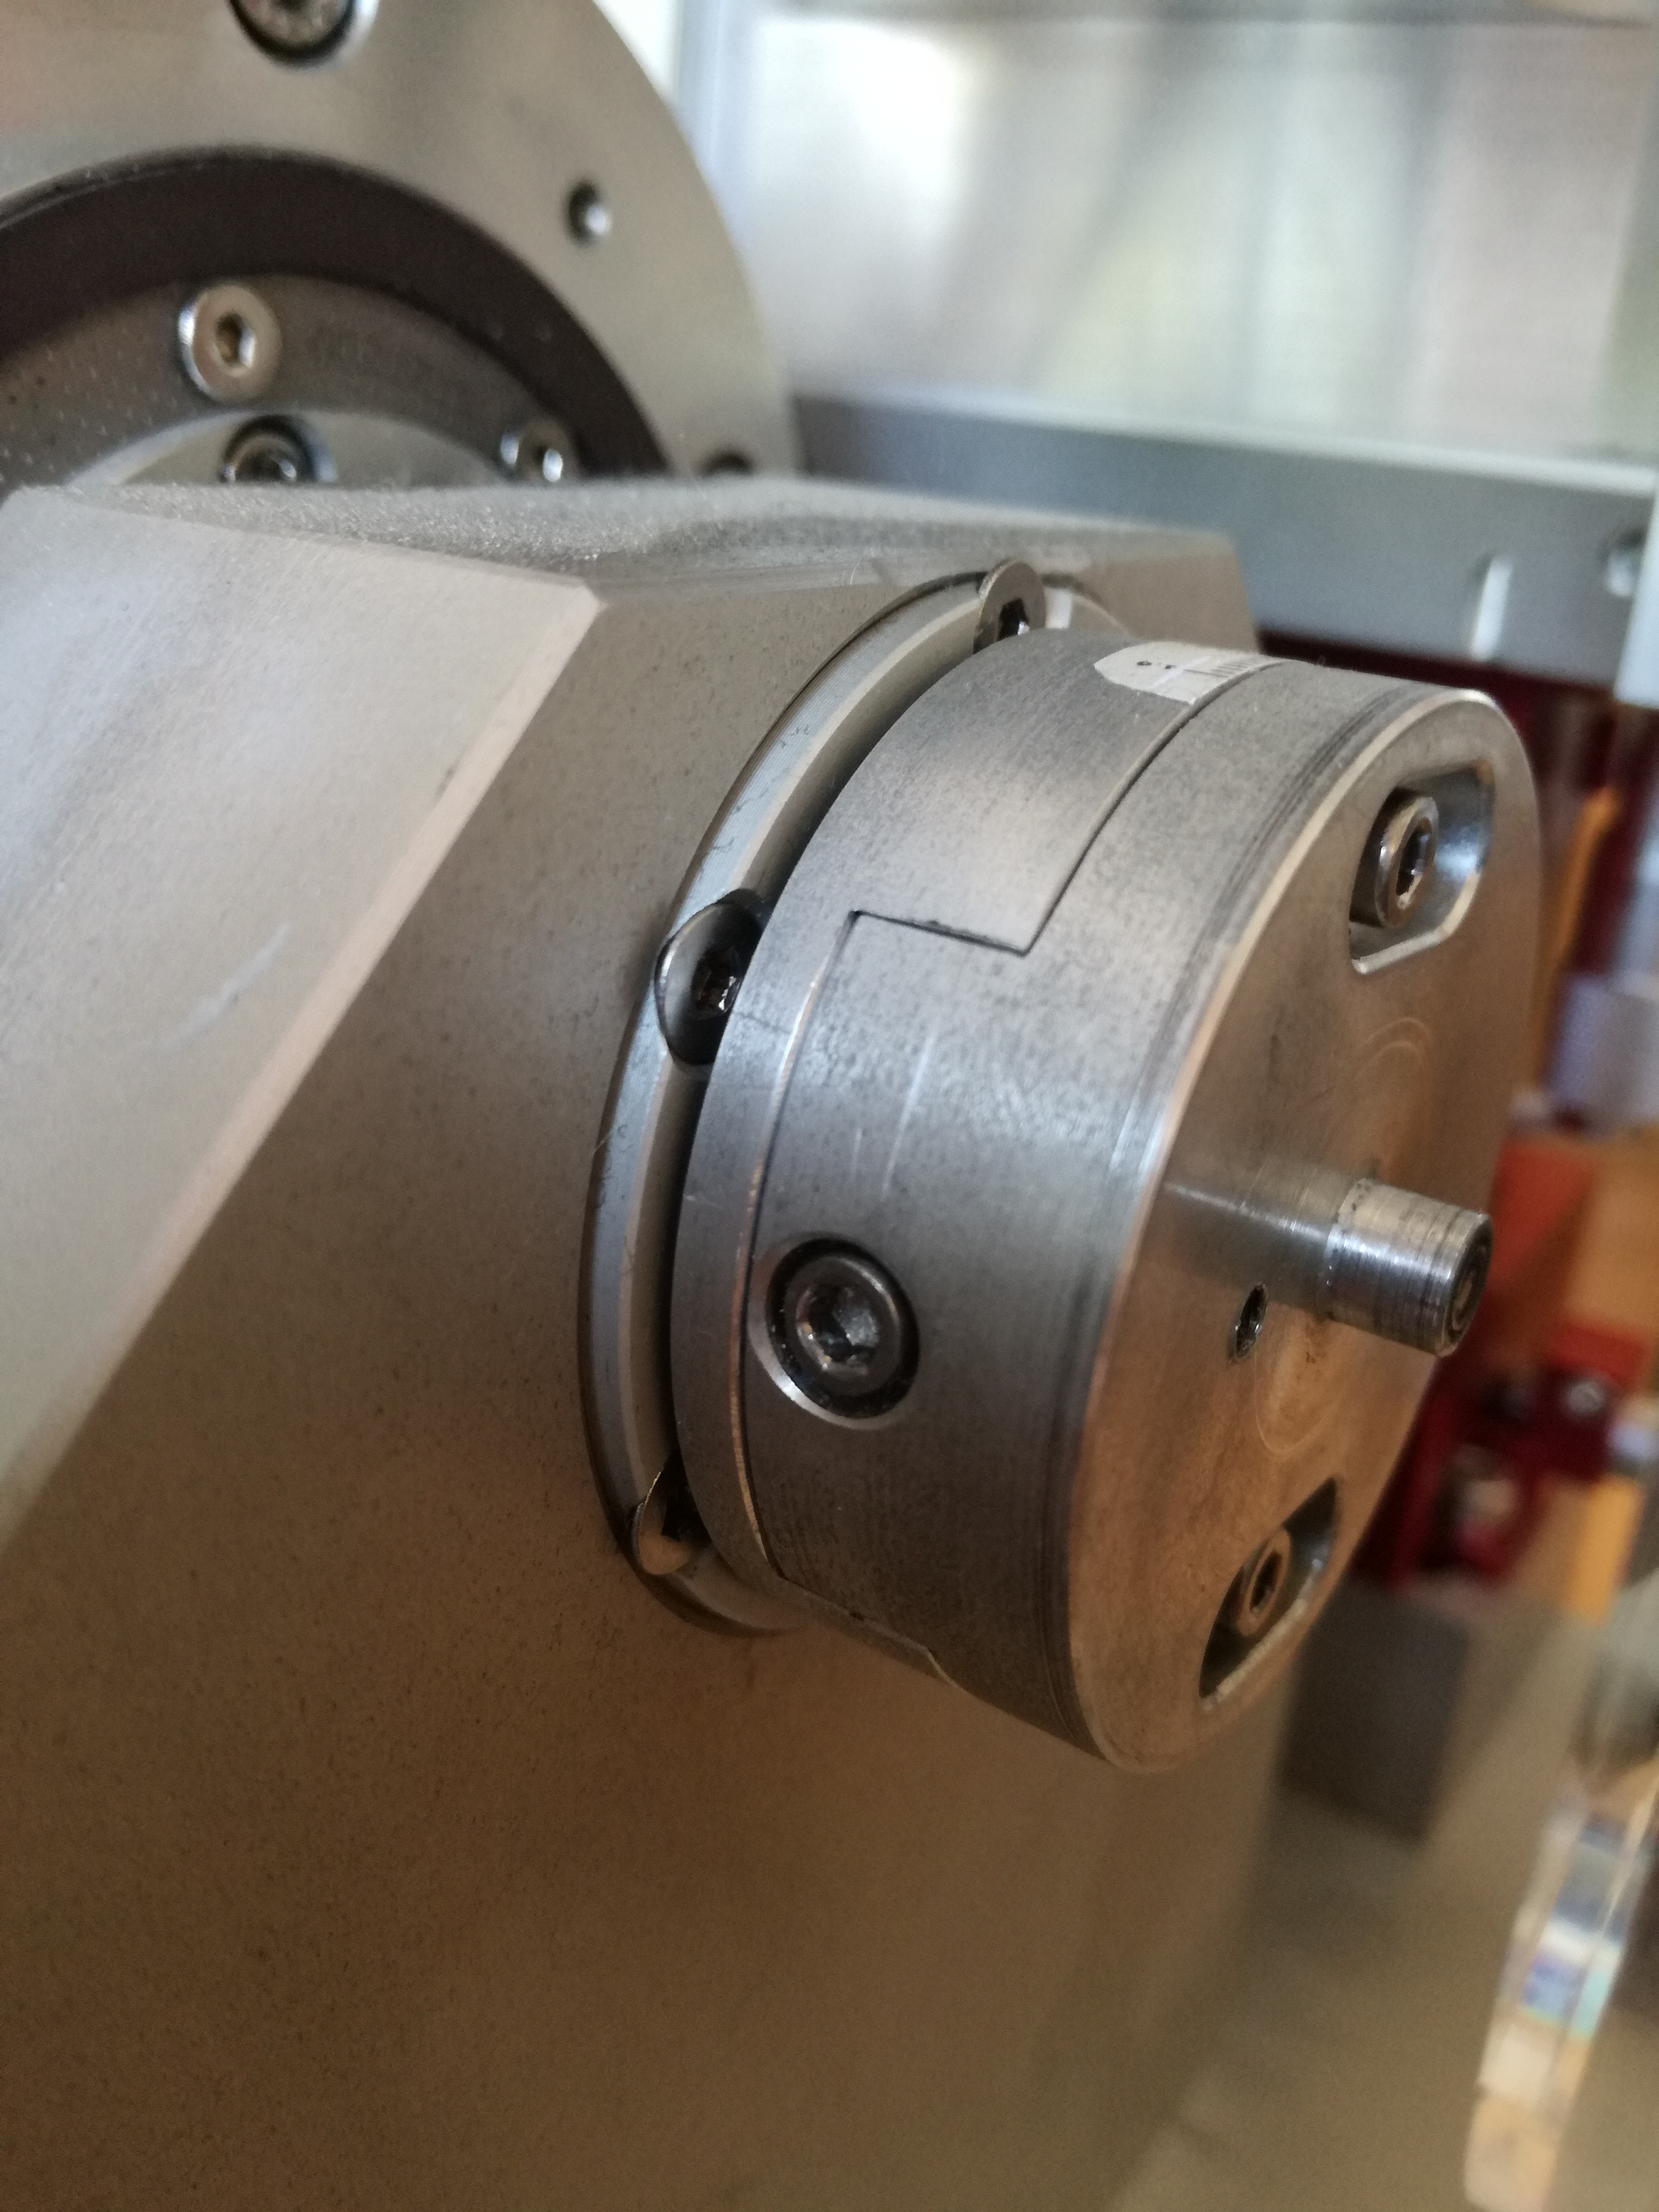
\includegraphics[width=0.4\columnwidth]{./Slike/premikanjeMagneta.jpg}
	\caption{Dinamično ekscentričnost se lahko izmeri le v eni smeri}
	\label{premikanjeMagneta}
\end{figure}
\begin{figure}[!ht]
	\centering
	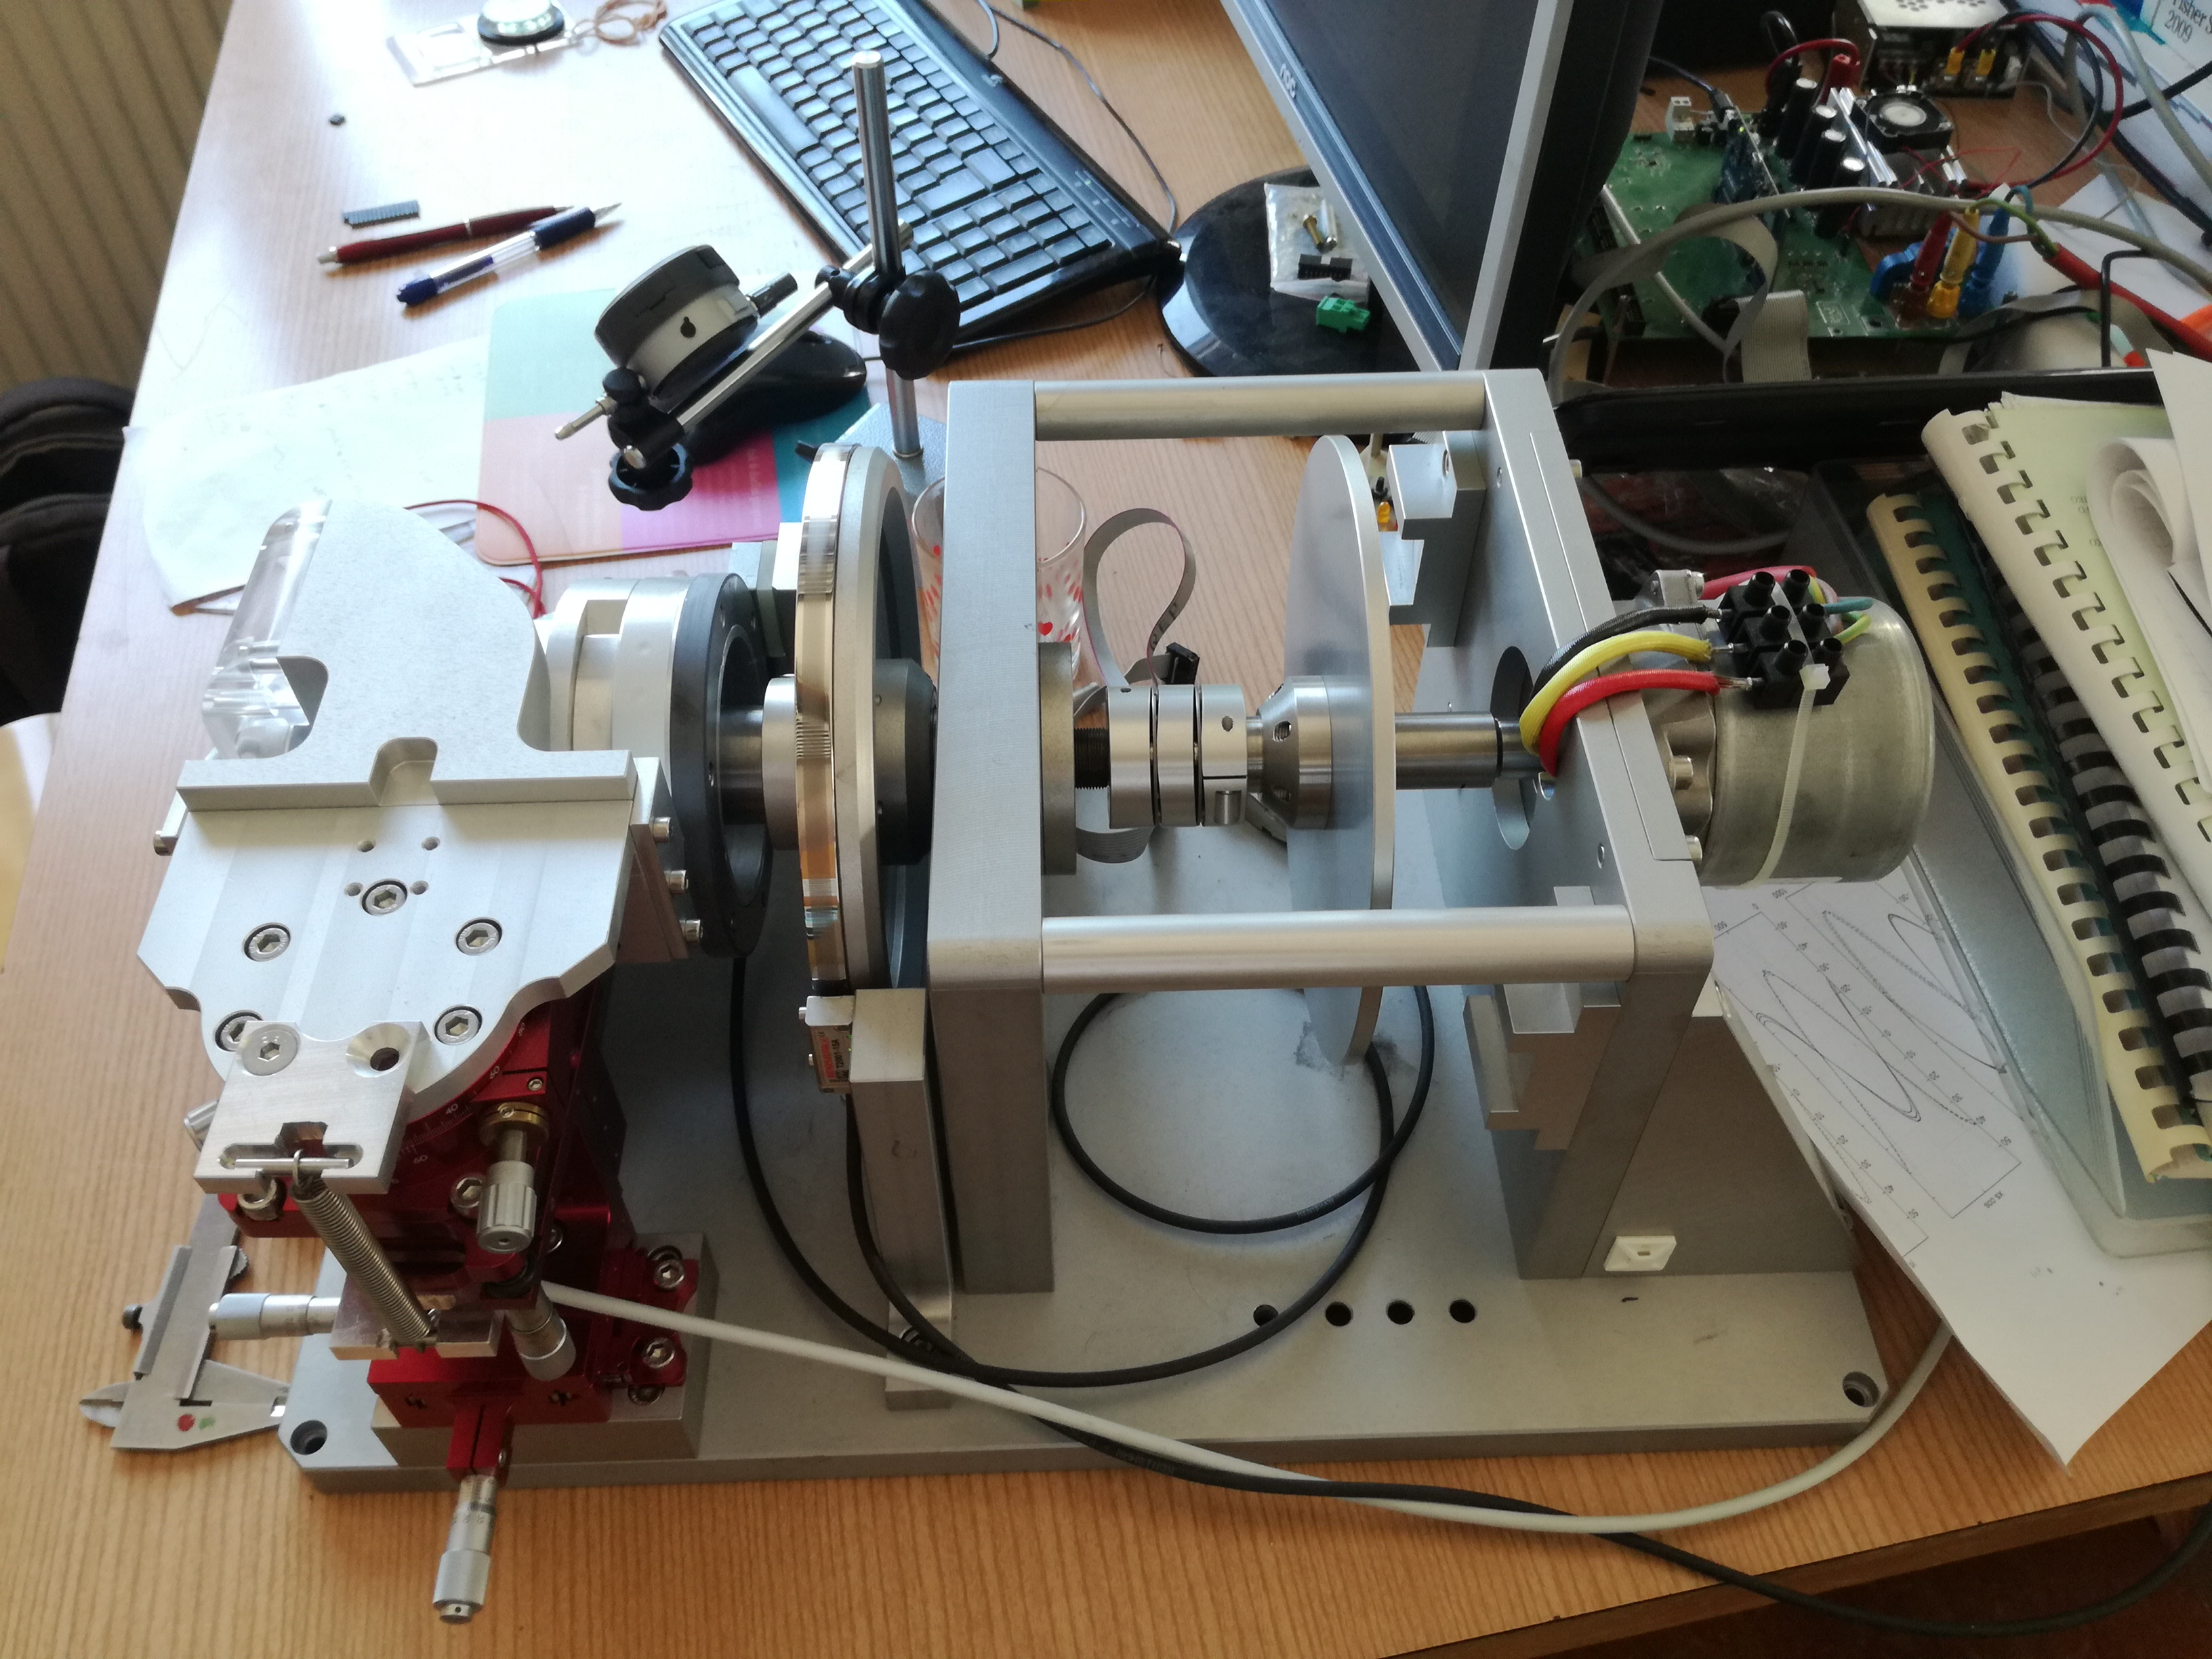
\includegraphics[width=0.75\textwidth]{./Slike/postavitevmerilnegamesta.jpg}
	\caption{Postavitev testnega mesta}
	\label{postavitevmerilnegamesta.jpg}
\end{figure}
\begin{figure}[!ht]
	\centering
	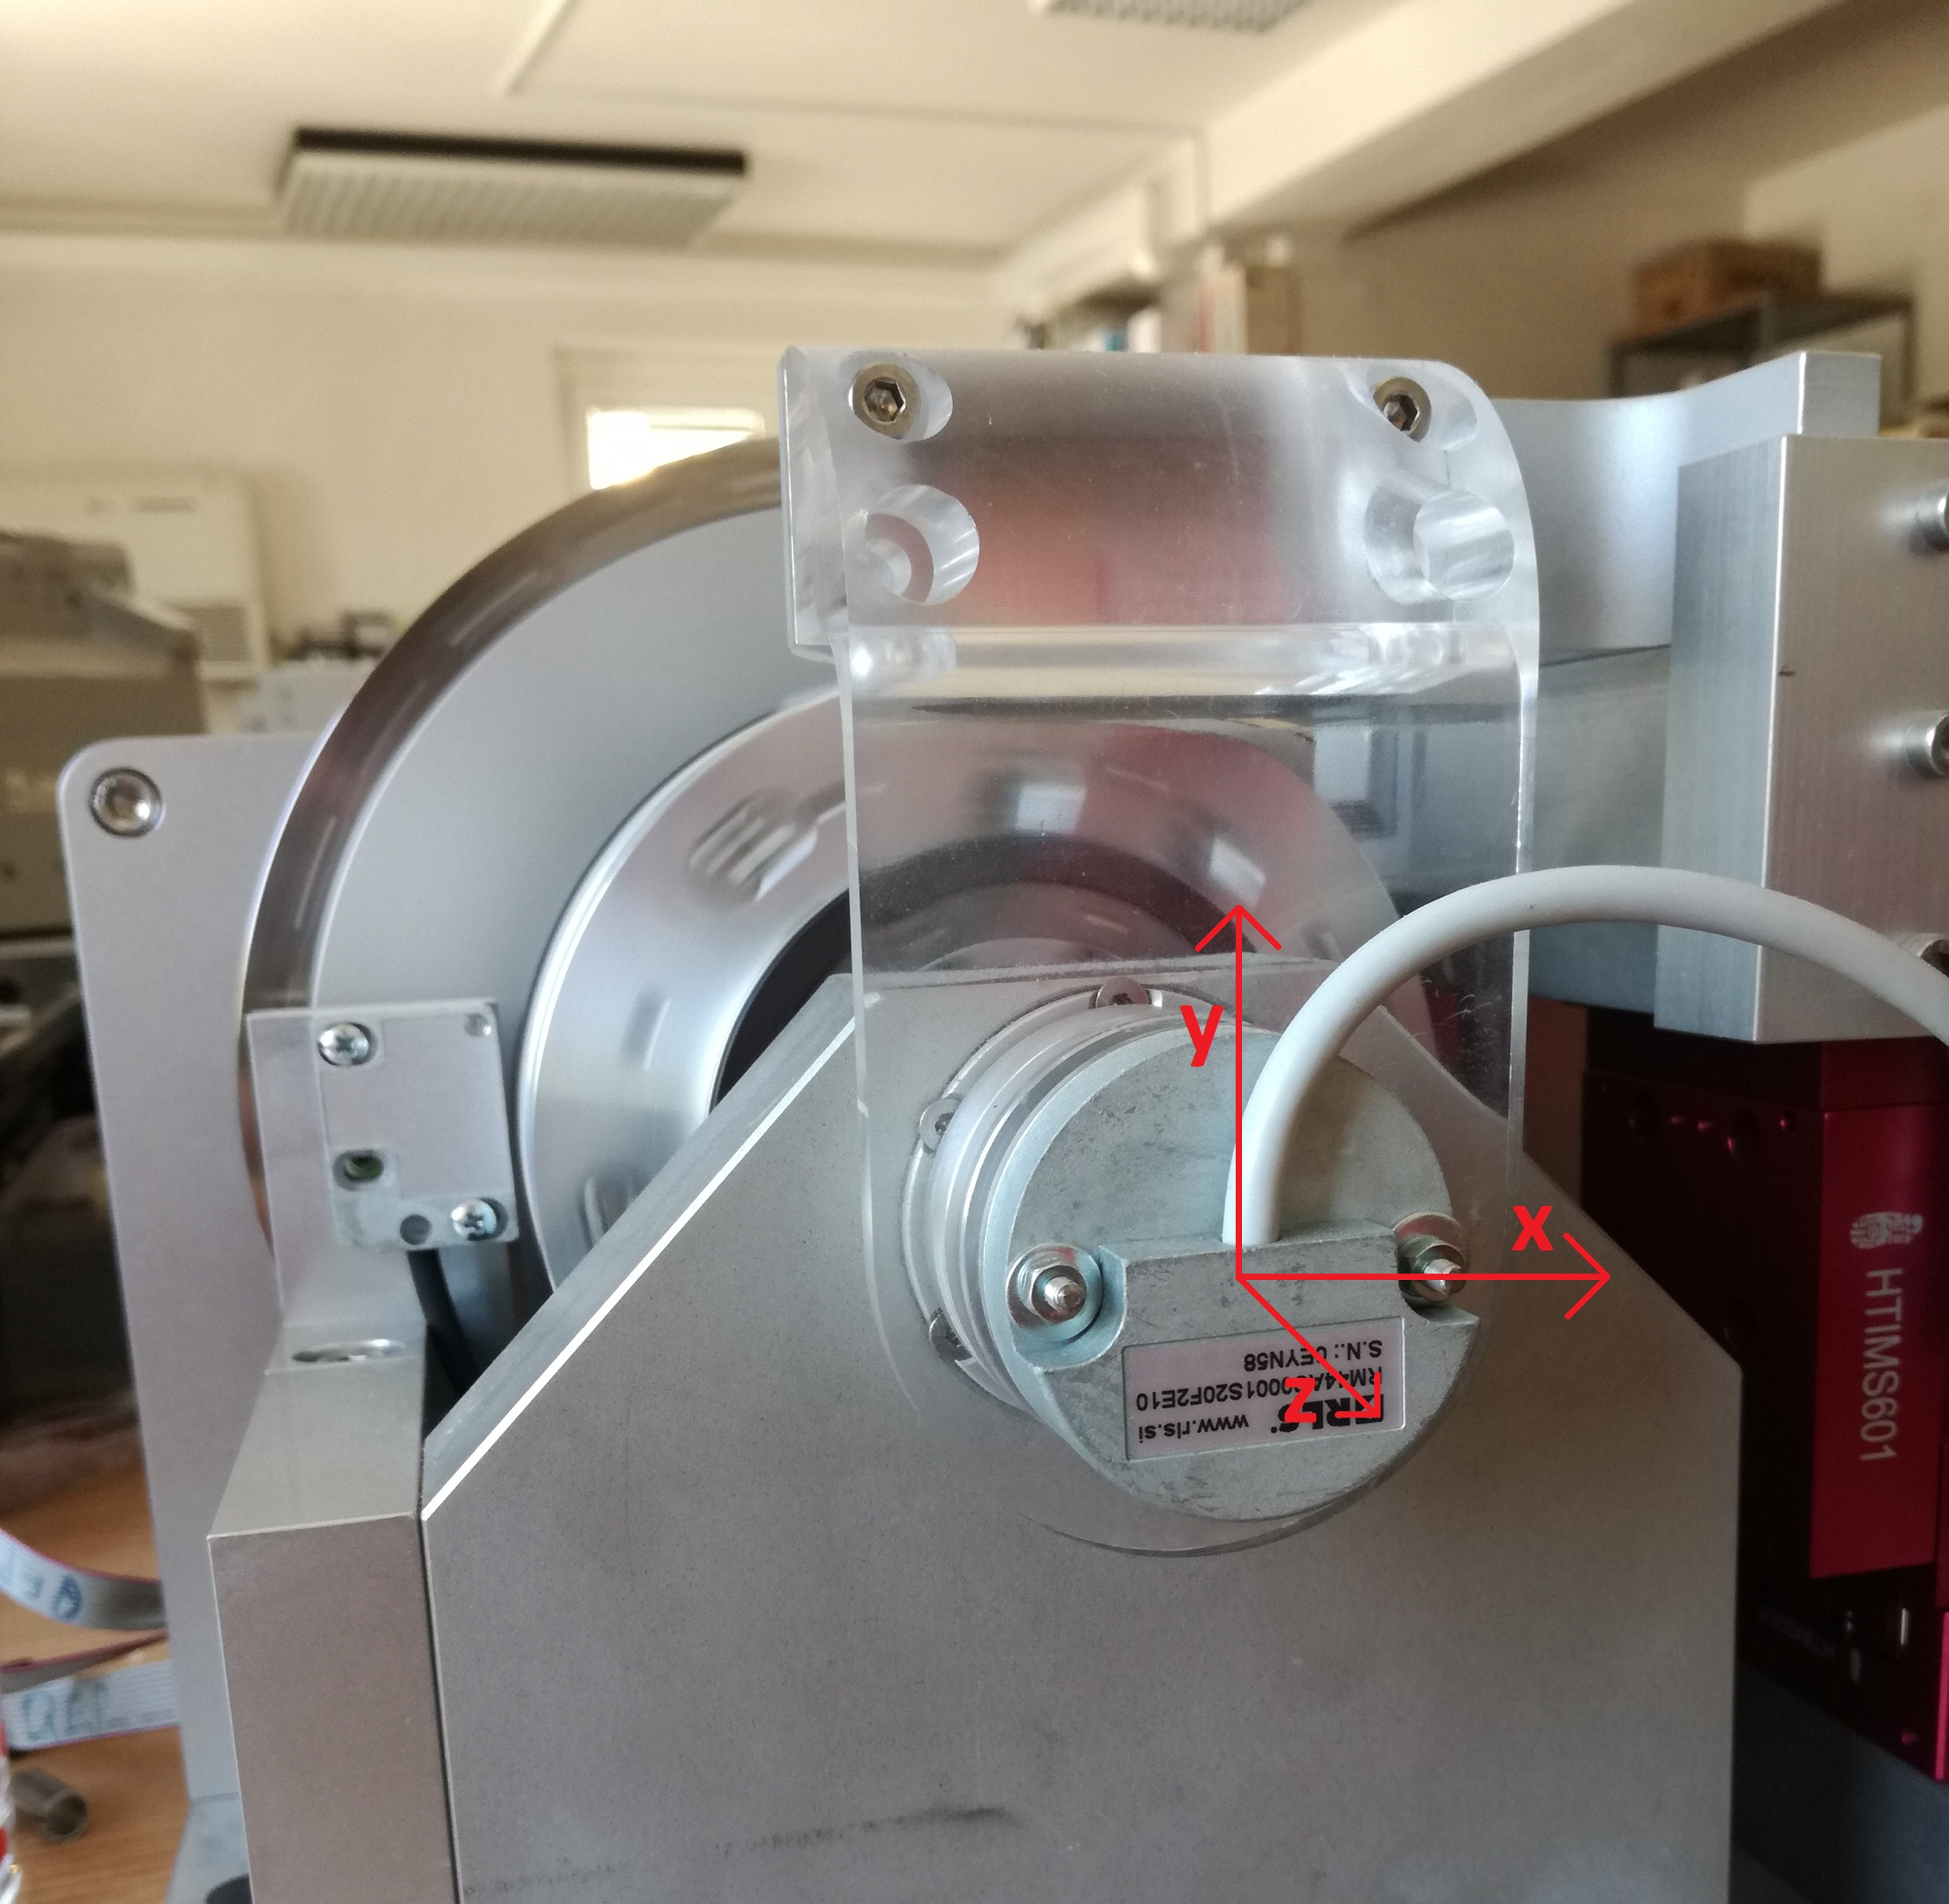
\includegraphics[width=0.65\textwidth]{./Slike/koordinatnisistem.jpg}
	\caption{Postavitev testnega mesta}
	\label{koordinatnisistem.jpg}
\end{figure}
\begin{figure}[!ht]
	\centering
	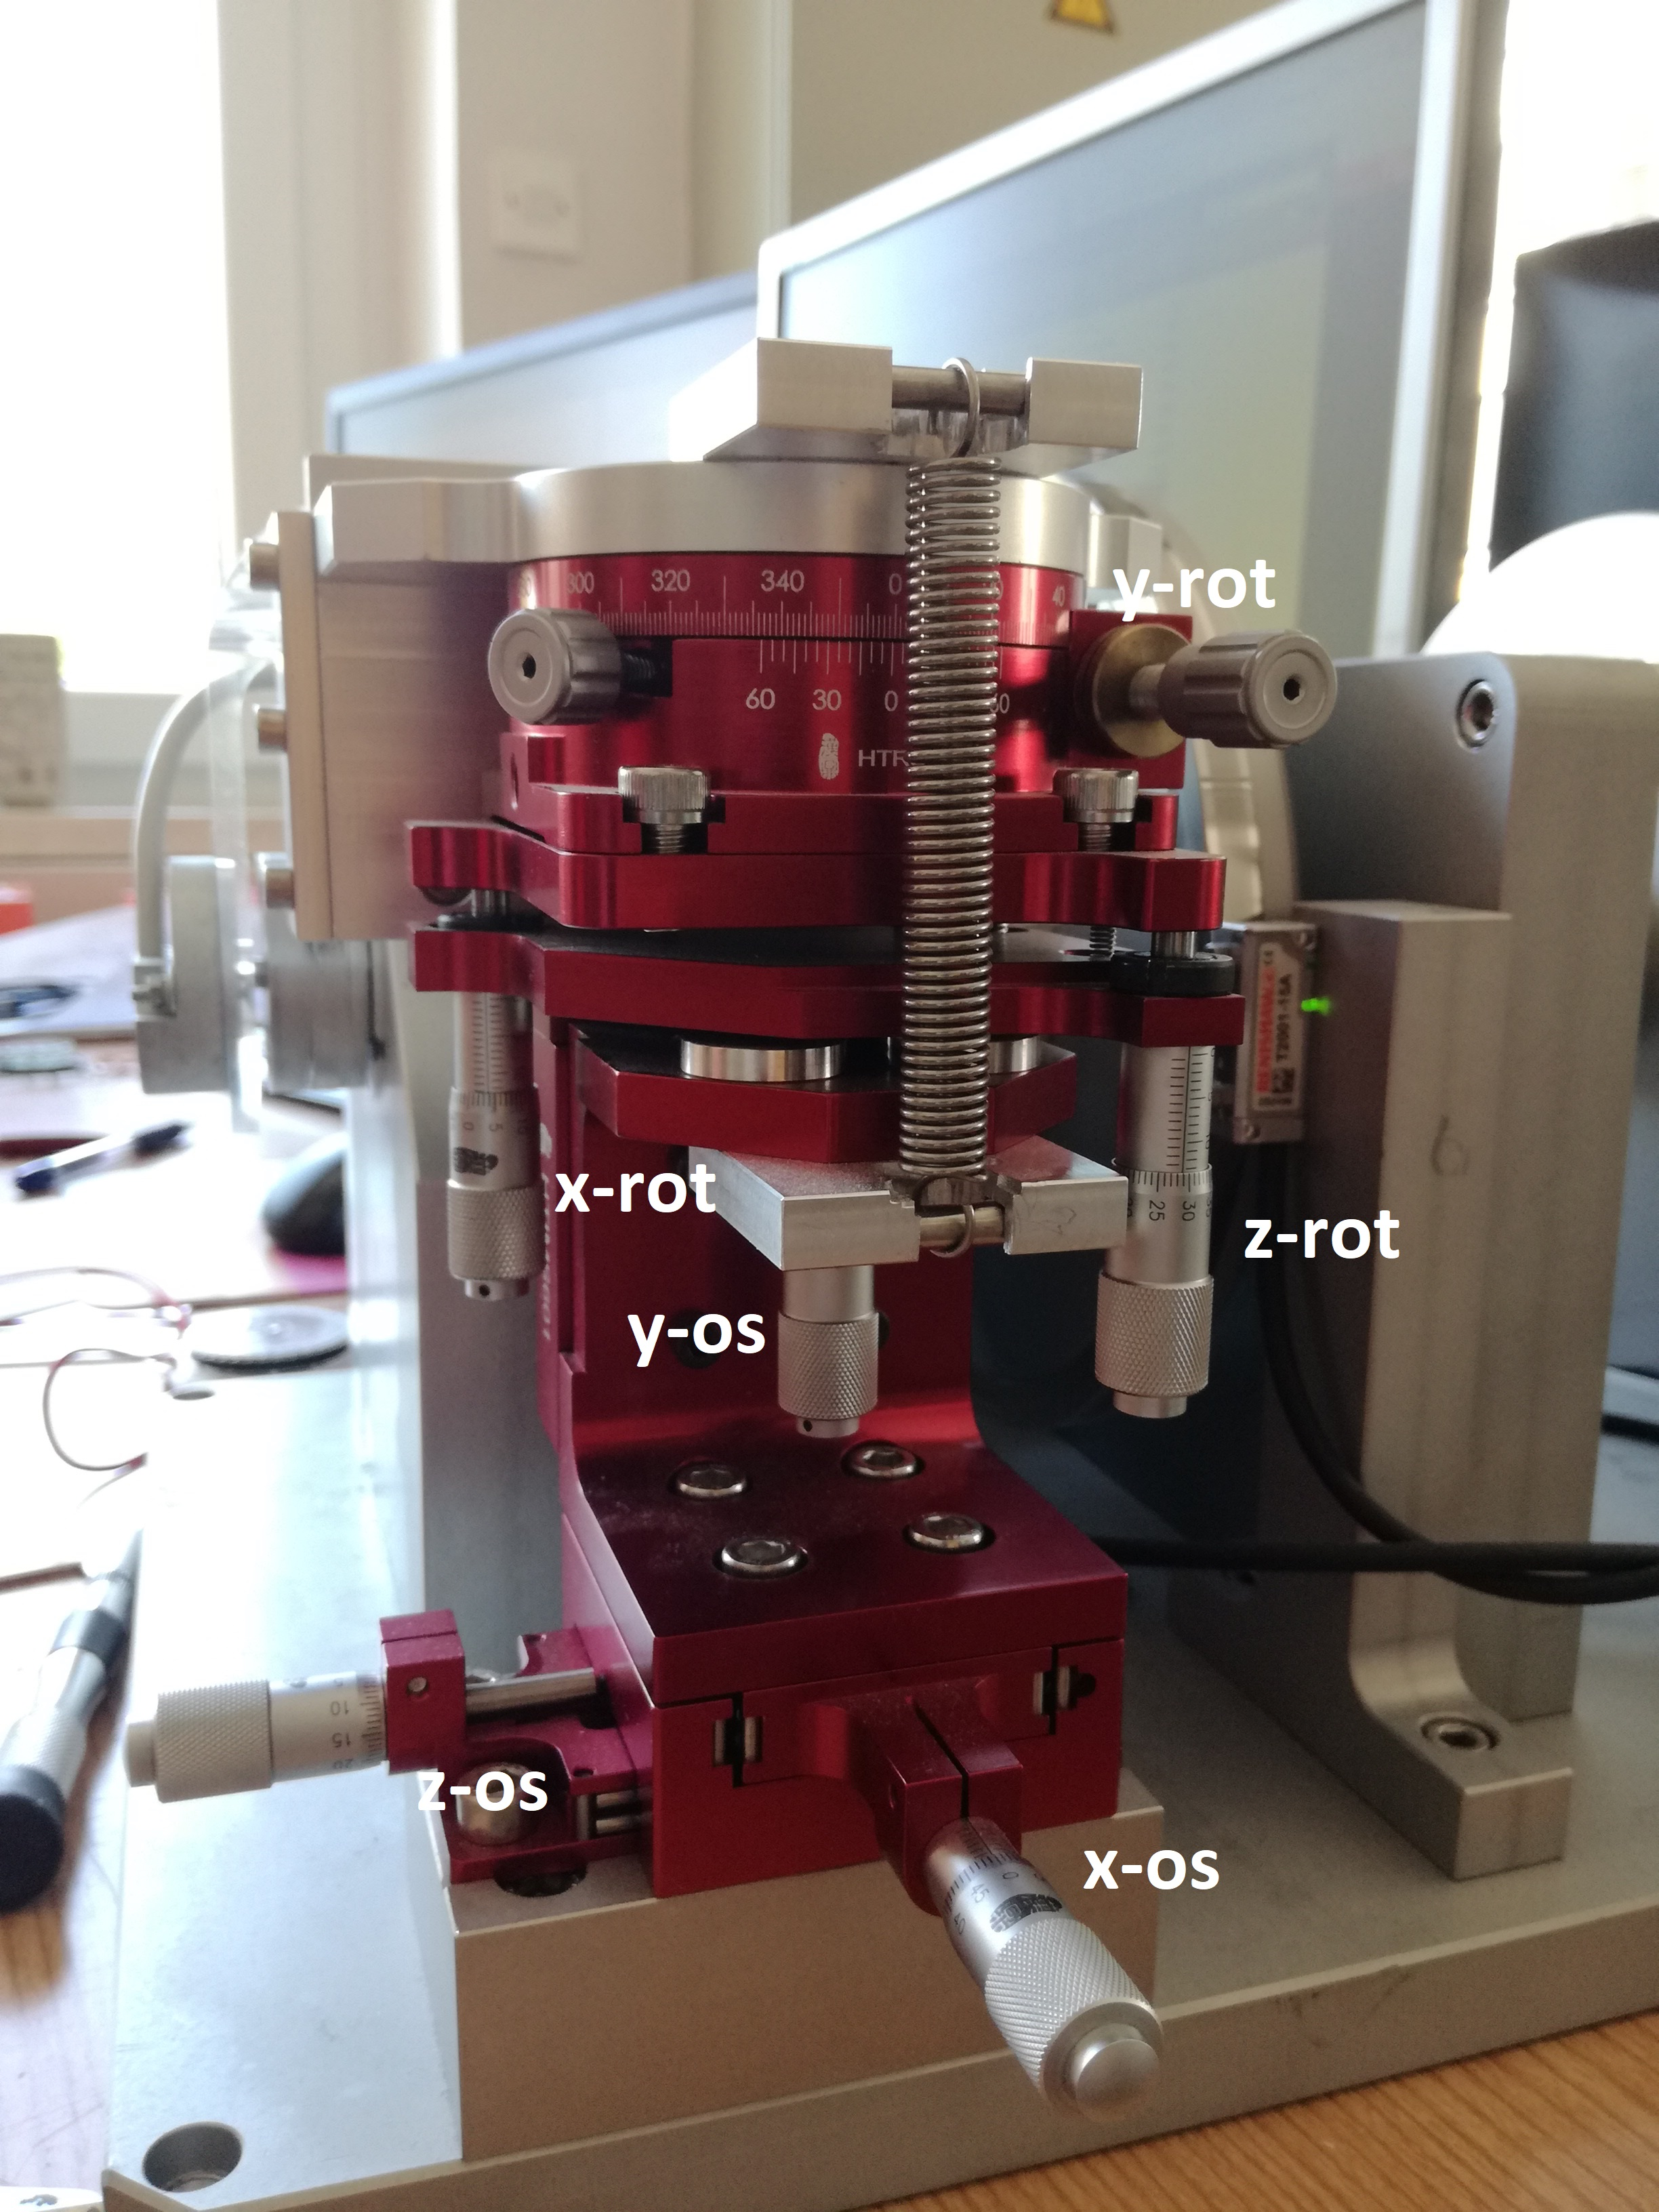
\includegraphics[width=0.55\textwidth]{./Slike/HTIMS601.jpg}
	\caption{Naprava za nastavljanje statične ekscentričnosti}
	\label{HTIMS601.jpg}
\end{figure}
Za manevriranje s HTIMS601 je potrebno nastaviti 6 osi.
S postavitvijo koordinatnega sistema (slika \ref{koordinatnisistem.jpg}), je vsak od vijakov definiral premik senzorja. 
Vsako os se nastavlja z enim od vijakov (slika \ref{HTIMS601.jpg}). Vijaki poimenovani x-os, y-os in z-os so za nastavljanje translaciijo merjenca, x-rot, y-rot in z-rot so za nastavljanje rotacije premikajoče plošče na vrhu HTIMS601.
S spremembo vrtenja vijakov translacijskih osi, se je lokacija senzorja pred magnetom spreminjala za enako spremembo. S spremembo vrtenja rotacijskih vijakov, se je zaradi ročice na katero je pritrjen senzor, senzor zarotira in hkrati tudi premakne iz dotedanje lege. S spremembo rotacije je potrebno popraviti tudi nastavitve vijakov, ki senzor premikajo v translacijskih oseh.

Hitrost vrtenja pogona je nastavljiva.
Hitrost vrtenja je pogona je nastavljena na 60 RPM. Hitrost ni popolnoma konstantna (slika \ref{hitrost}). Vzrok je v vztrajnosti pogona. Mitja Nemec je problem skušal čimbolje odpraviti, z dodajanjem primernih uteži na primerna mesta na vztrajniku.
\slikaeps{Potek hitrosti od zasuka}{hitrost}
\newpage
\section{Zajem podatkov}
Mitja Nemec je pripravil grafični uporabniški vmesnik za prikazovanje meritev (slika \ref{GUI.png}).
Vmesnik lahko prikazuje potek refernečnega kota, $B_{sin}$ in $B_{cos}$ senzorja RM44, izračunanega kota iz $B_{sin}$ in $B_{cos}$ signala, napako med izračunanim kotom senzorja in refernčnim dajalnikom, hitrost vrtenja ter tok prve faze motorskega pogona. Signaloma $B_{sin}$ in $B_{cos}$ se v programu prišteje enosmerna komponenta, ki bi popravila signala.

Krmilna plošča (slika \ref{krmilnaplosca.jpg}) zajema podatke pogona s frekvenco 1kHz.
Referenčni inkrementalni dajalnik, se ob zagonu inicializira. V programu se podatek o kotu deli z 12595200. Definicijsko območje referenčnega kota se giblje med 0 in 1.
Signala $B_{sin}$ in $B_{cos}$  se na krmilni plošči ojačata in pretvorita z 12 bitnim AD pretvornikom. Izhod AD pretvornika se odšteje 2048 in deli s 4096. Definicijsko območje  $B_{sin}$ in $B_{cos}$  signala se gibljeta med $\pm0,5$.
Hitrost in napaka sta izračunana iz zajetih signalov.
Podatki so v obliki enega paketa poslani s krmilne plošče na 1 sekundo. Pri frekvenci vrtenja 1 Hz, grafični vmesnik prikaže en obrat.
Podatke se lahko izvozi v obliki .csv datoteke in nato poljubno obdela.
Na sliki  \ref{GUI.png} je prikazan sinusni signal prikazan kot da je zamaknjen za 180$\mathrm{^\circ}$. To je posledica definicije pozitvne smeri vrtenja za senzor \cite{RM44}. Senzor ima nasproto definirano pozitivno smer vrtenja. To sem rešil tako, da sem obrnil podatke. Popraviti je bilo potrebno tudi potek referenčnega dajalnika.
\begin{figure}[!ht]
	\centering
	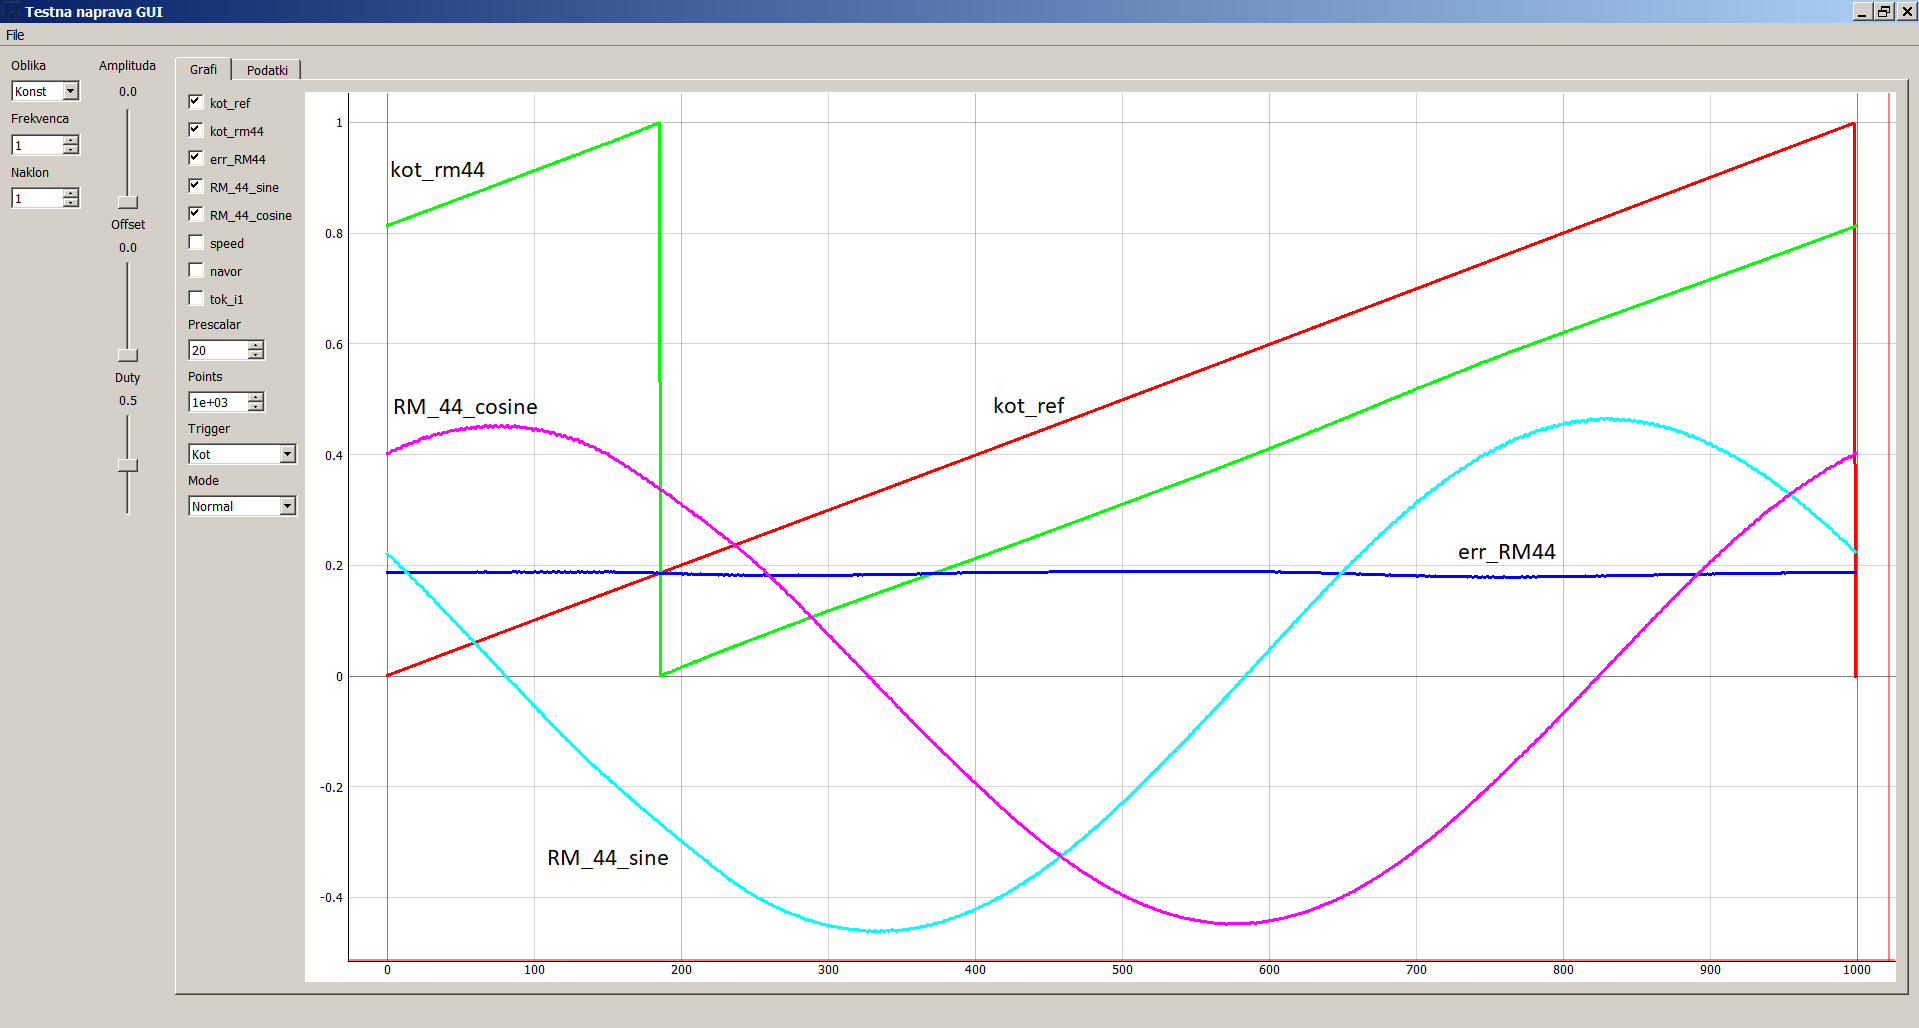
\includegraphics[width=0.99\textwidth]{./Slike/GUI.png}
	\caption{Grafični vmesnik s poteki signalov}
	\label{GUI.png}
\end{figure}

\begin{figure}[!ht]
	\centering
	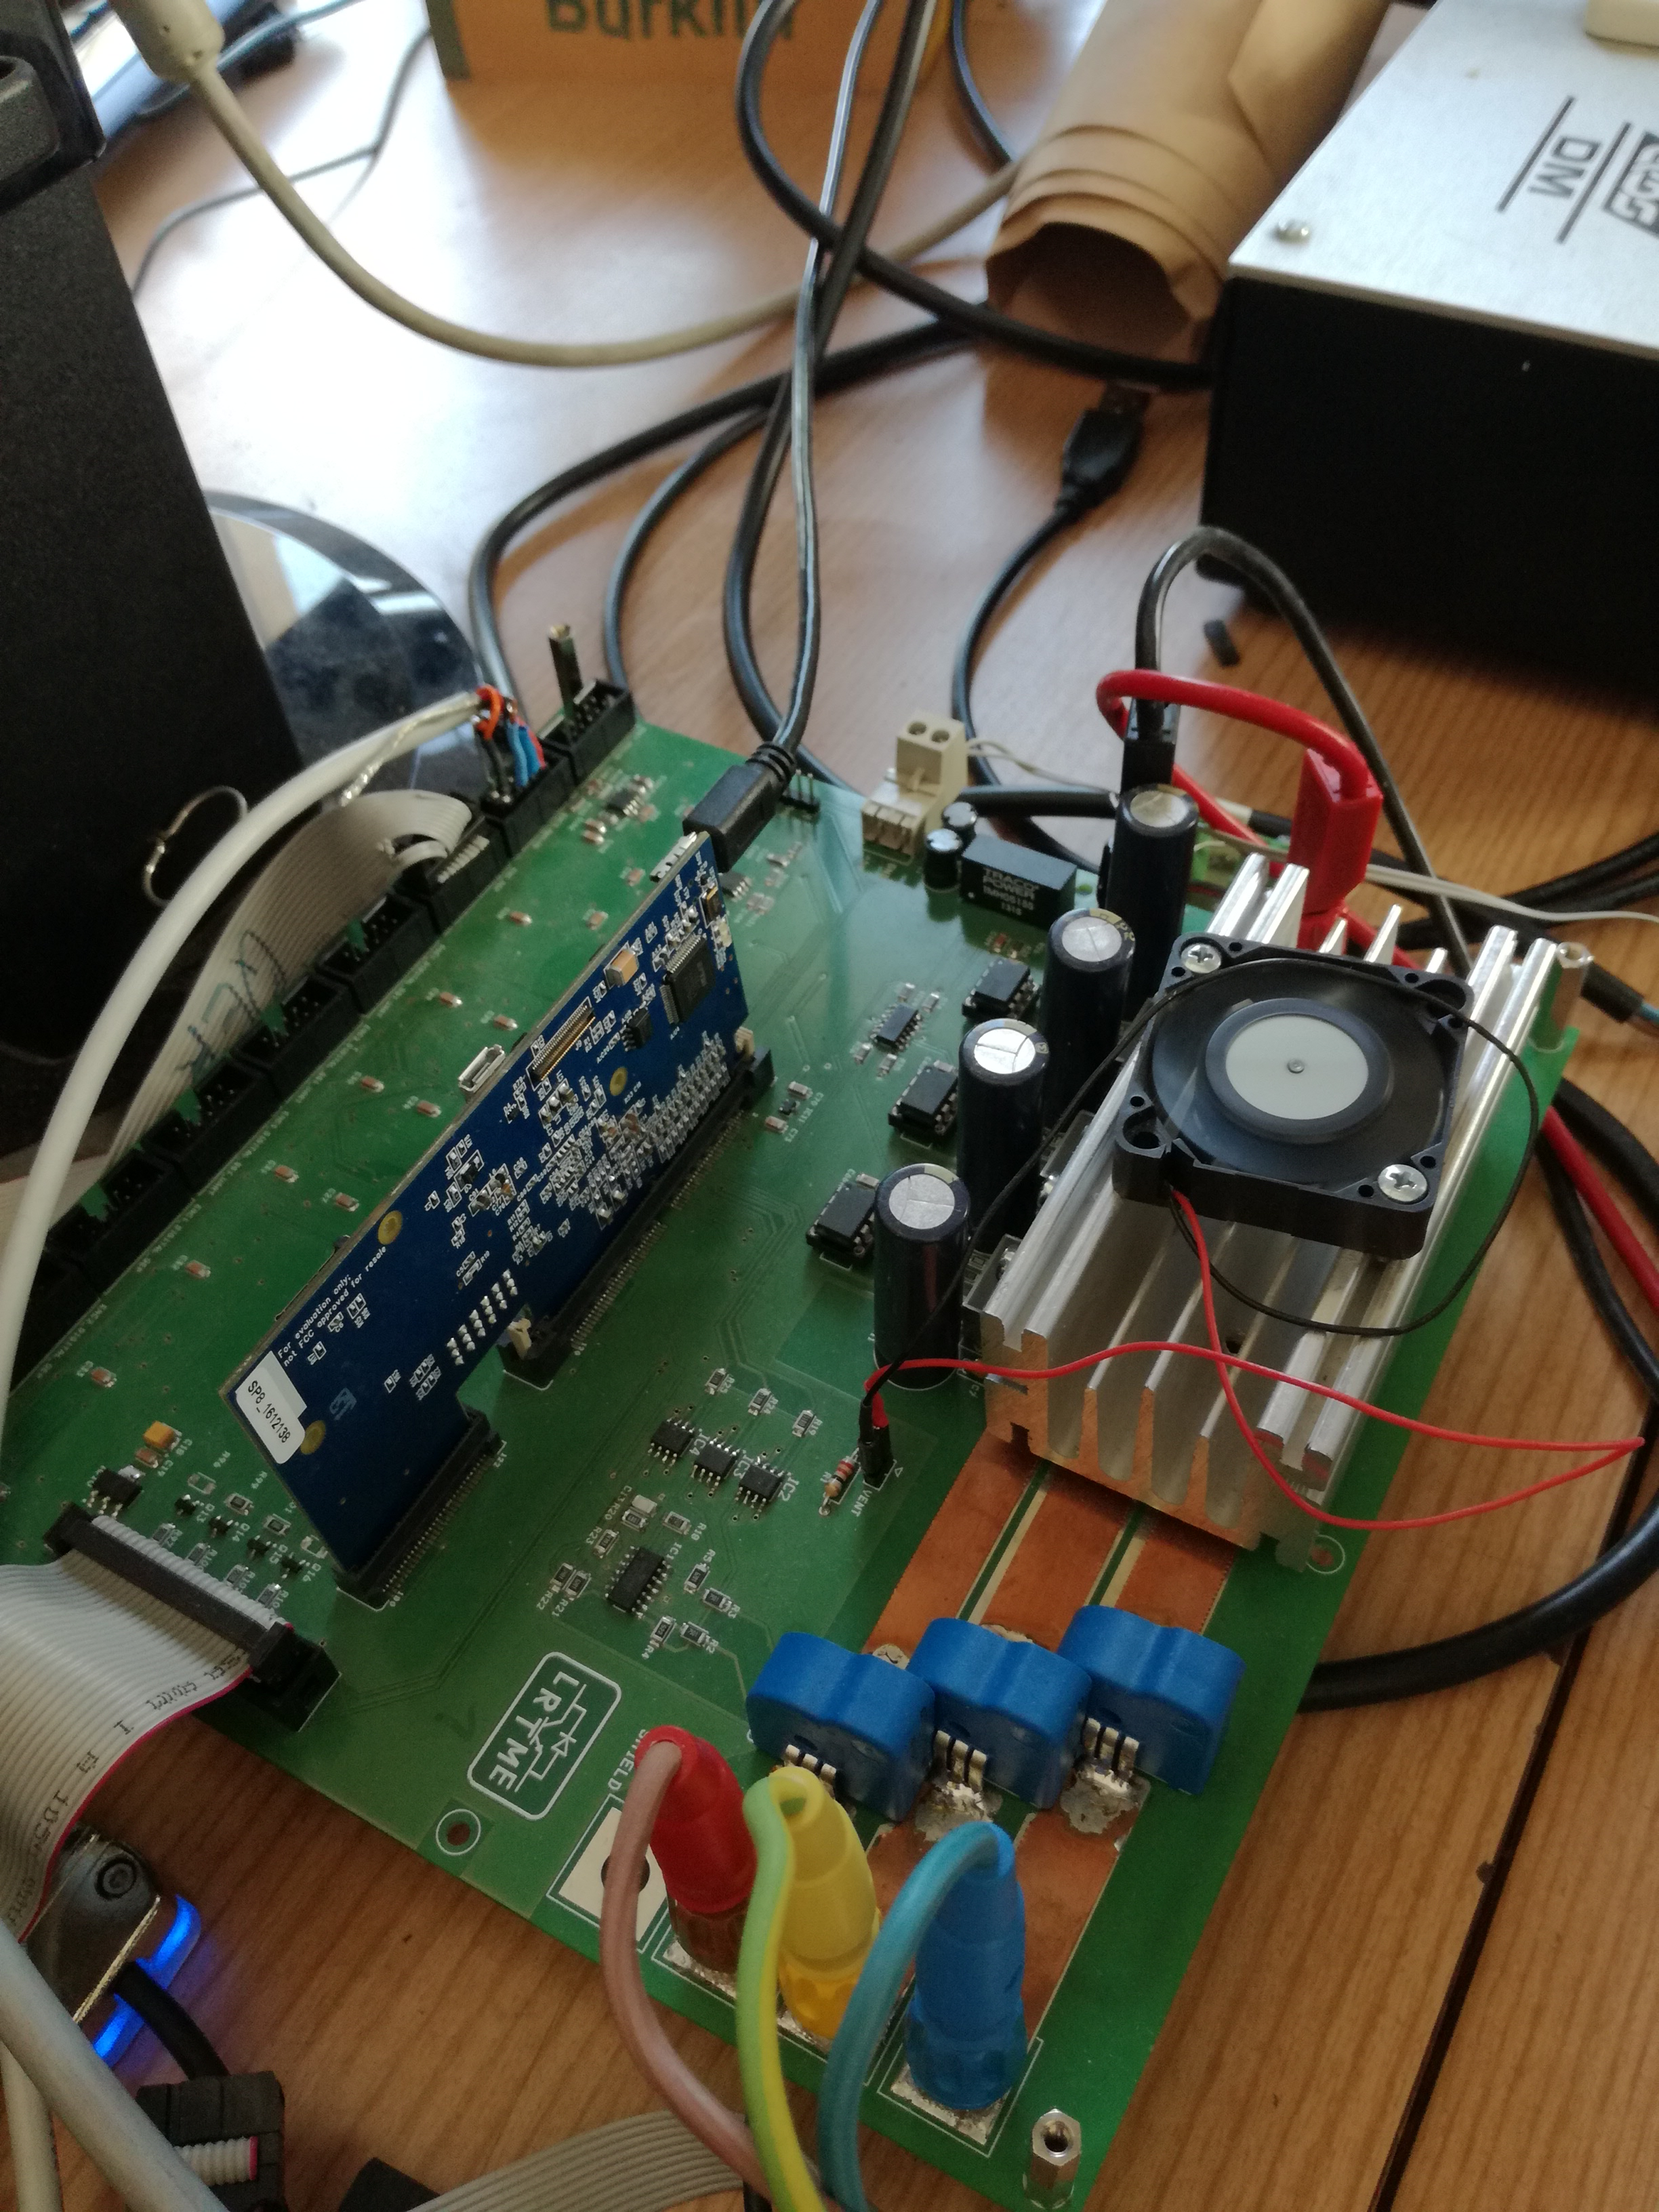
\includegraphics[width=0.55\textwidth]{./Slike/krmilnaplosca.jpg}
	\caption{Krmilna plošča za krmiljenje pogona in obdelavo signalov s dajalnikov položaja}
	\label{krmilnaplosca.jpg}
\end{figure}
\newpage
\section{Senzor v izhodiščni legi}
Senzor in magnet se lahko gibljeta, najprimernejša, izhodiščna lega, ni definirana. Z merilno urico Mitutoyo 543-391B se je dinamično ekscentričnost magneta nastavilo na najmanjšo. Oplet z merilno urico je bil pomerjen $\pm 3 \mathrm{\mu m}$.
S prilagajanjem vijakov HTIMS601, opazovanjem $B_{sin}$ in $B_{cos}$ ter napake je bil senzor nastavljen v lego, kjer je bila amplituda drugega harmonika napake najmanjša. Najprimernejšo lego sem iskal glede na vrednost amplitud in ortogonalnost  $B_{sin}$ in $B_{cos}$. Signala $B_{sin}$ in $B_{cos}$ morata ustrezati definicijskem območju zajema AD pretvornika.

Na sliki \ref{./MER/00_sincos} sta prikazana $B_{sin}$ in $B_{cos}$. Enosmerni komponenti sta prisotni v obeh signalih, posledično se izrazi v napaki prvi harmonik (slika \ref{./MER/00_napaka}).
V napaki se pojavi med $\mathrm{95^\circ}$ in $\mathrm{140^\circ}$ preskok napake. Vzroka nisem raziskoval.
Z razvojem napake v Fourierovo vrsto (slika \ref{./MER/00_fft}) vidimo velikosti posameznih amplitud napake.
Enosmerna komponenta je posledica sofaznih zamikov obeh signalov $B_{sin}$ in $B_{cos}$. 
Prvi harmonik je posledica ensmermih komponent $B_{sin}$ in $B_{cos}$. Z matematično obdelavo siganlov $B_{sin}$ in $B_{cos}$ sem enosmerni komponenti odstranil,vendar se prvi harmonik napake še vedno izrazi. Prvi harmonik napake je odvisen tudi od drugega harmonika v signalih $B_{sin}$ in $B_{cos}$.
Z odstranitvijo tudi drugega harmonika iz signalov $B_{sin}$ in $B_{cos}$ je bil  prvi harmonik v napaki odstranjen.
Signala  $B_{sin}$ in $B_{cos}$ med izvajanjem meritev ne bosta  matematično obdelana. Spreminjanje signalov  $B_{sin}$ in $B_{cos}$ in napake se bo opazovalo glede na potek, ki je bil pomerjen v izhodiščni legi.
\slikaeps{Signala $B_{sin}$ in $B_{cos}$ pomerjena v izhodiščni legi}{./MER/00_sincos}
\slikaeps{Napaka $\varepsilon$ pomerjena v izhodiščni legi}{./MER/00_napaka}
\slikaeps{Amplitude harmonikov napake $\varepsilon$ razvite v Fourierovo vrsto pri meritvah v izhodiščni legi}{./MER/00_fft}
\newpage

\subsection{Meritve v izhodišni legi}
V izhodiščni legi je bilo opravljenih več meritev. Osredotočil sem se na enosmerni komponenti  in amplitudi osnovnega harmonika $B_{sin}$ in $B_{cos}$. 
Porazdelitev enosmerne komponente signala $B_{sin}$ in $B_{cos}$ je prikazana na sliki \ref{./MER/00_off}.
Srednja vrednost enosmerne komponente $B_{sin}$ je $-8,85 \cdot 10^{-4}$, standardna deviacija je $1,08\cdot 10^{-4}$.
Srednja vrednost enosmerne komponente $B_{cos}$ je $4,20 \cdot 10^{-3}$, standardna deviacija je $5,20\cdot 10^{-5}$.
\slikaeps{Porazdelitev meritev enosmerne komponente signalov $B_{sin}$ in $B_{cos}$}{./MER/00_off}
Porazdelitev amplitude osnovnega harmonika signala $B_{sin}$ in $B_{cos}$ je prikazana na sliki \ref{./MER/00_off}.
Srednja vrednost amplitude osnovnega harmonika $B_{sin}$ je $0,451$, standardna deviacija je $2,20\cdot 10^{-4}$.
Srednja vrednost amplitude osnovnega harmonika $B_{cos}$ je $0,449$, standardna deviacija je $1,95\cdot 10^{-4}$.
\slikaeps{Porazdelitev meritev amplitude osnovnega harmonika signalov $B_{sin}$ in $B_{cos}$}{./MER/00_amp}
\newpage
\section{Meritve statične ekscentričnosti v smeri x-osi}
Pri meritvi je pričakovati spremembo amplitud in faznih zamikov signalov $B_{sin}$ in $B_{cos}$. Na sliki \ref{./MER/xs_sincos} sta prikazana $B_{sin}$ in $B_{cos}$ pomerjena pri 0,20 mm statične ekscentričnosti v smeri x. Na signalih, med 95 in 175$^\circ$ se pojavijo nenavadni skoki.
Izrazijo se tudi na napaki, ki je prikazana na sliki \ref{./MER/xs_napaka}. Vzrok tega pojava nisem raziskoval. Napaka razvita v Fourierovo vrsto prikaže pričakovano povišanje drugega harmonika.
\slikaeps{Signala $B_{sin}$ in $B_{cos}$ merjena pri 0,2 mm statične ekscentičnosti v smeri x}{./MER/xs_sincos}
\slikaeps{Napaka $\varepsilon$ merjena pri 0,2 mm statične ekscentičnosti v smeri x}{./MER/xs_napaka}
\slikaeps{Amplitude harmonikov napake $\varepsilon$ razvite v Fourierovo vrsto merjeno pri 0,2 mm statične ekscentičnosti v smeri x}{./MER/xs_fft}
\newpage
\subsection{Sprememba signalov Hallovih sond ter napake v odvisnosti od statične ekscentričnosti v smeri x}
Iz simulacij se pričakuje hitrejše spreminjanje amplitude osnovnega harmonika $B_{cos}$ signala. Sprememba amplitud osnovnih harmonikov je prikazana na sliki \ref{./MER/xs_sincos_amp}. Amplituda signala $B_{cos}$ pada, pada tudi ampituda signala $B_{sin}$. Signala nimata enake amplitude v izhodišču, kar je posledica neidealne izhodiščne lege. Potek enosmerne komponente je prikazan na sliki \ref{./MER/xs_sincos_off}. Fazni zamik signalov je prikazan na sliki \ref{./MER/xs_sincos_phase}. Pričakovano po simulacijah se fazna razlika med signaloma zmanjšuje. Pri meritvah se je fazni kot $B_{cos}$ zmanjševal, fazni kot $B_{sin}$ naraščal. Razlika med njima je manjša, kot je bila posimulirana. Vsota faznih zamikov ostaja konstantna, zato se enosmerna komponenta v napaki ne spreminja.
Poteki posameznih komponent signalov $B_{sin}$ in $B_{cos}$ so aproksimirani s kubičnimi polinomi.
\begin{eqnarray}
&\begin{split}Off_{sin} (\Delta x_s) =-3,88\cdot 10^{-2}\Delta x_s^{3}+2,37\cdot 10^{-2}\Delta x_s^{2}-2,25\cdot 10^{-3}\Delta x_s\\-9,53\cdot 10^{-4} \end{split}\\
&\begin{split}A_{sin}(\Delta x_s) =-6,14\cdot 10^{-2}\Delta x_s^{3}-1,71\cdot 10^{-2}\Delta x_s^{2}-1,17\cdot 10^{-2}\Delta x_s\\+4,84\cdot 10^{-1} \end{split}\\  
&\delta_{sin} (\Delta x_s) =5,32\Delta x_s^{3}-3,55\Delta x_s^{2}+3,49\Delta x_s+1,08 \\                                                  
&\begin{split}Off_{cos} (\Delta x_s) =2,21\cdot 10^{-2}\Delta x_s^{3}-1,91\cdot 10^{-2}\Delta x_s^{2}-3,91\cdot 10^{-3}\Delta x_s\\+6,48\cdot 10^{-3} \end{split}\\ 
&\begin{split}A_{cos} (\Delta x_s) =7,46\cdot 10^{-3}\Delta x_s^{3}-1,85\cdot 10^{-1}\Delta x_s^{2}+1,01\cdot 10^{-2}\Delta x_s\\+4,88\cdot 10^{-1} \end{split}\\   
&\delta_{cos} (\Delta x_s) =1,15\cdot 10\Delta x_s^{3}-1,06\cdot 10\Delta x_s^{2}-1,14\Delta x_s+1,19
\end{eqnarray}
\slikaeps{Potek amplitude osnovnega harmonika $B_{sin}$ in $B_{cos}$ pri meritvah statične ekscentričnosti v smeri x}{./MER/xs_sincos_amp}
\slikaeps{Potek enosmerne komponente $B_{sin}$ in $B_{cos}$ pri meritvah statične ekscentričnosti v smeri x}{./MER/xs_sincos_off}
\slikaeps{Fazni zamik osnovnega harmonika  $B_{sin}$ in $B_{cos}$ pri meritvah statične ekscentričnosti v smeri x  glede na idealna signala $B_{sin}$ in $B_{cos}$}{./MER/xs_sincos_phase}


Slika \ref{./MER/xs_potek} prikazuje poteke amplitud posameznih harmonikov napake v odvisnosti od statične ekscentričnosti v smeri x. Kvadratično narašča amplituda drugega harmonika, medtem ko so enosmerna komponenta in ostali harmoniki konstantni. Poteki so aproksimirani s kubičnimi polinomi.
\slikaeps{Potek amplitud posameznega harmonika napake $\varepsilon$ pri meritvah statične ekscentričnosti v smeri x}{./MER/xs_potek}
\begin{eqnarray}
&C_0(\Delta x_s) =2,42\Delta x_s^{3}-1,71\Delta x_s^{2}+2,40\cdot 10^{-1}\Delta x_s+1,15 \\              
&C_1(\Delta x_s) =-3,01\Delta x_s^{3}+2,35\Delta x_s^{2}-6,35\cdot 10^{-1}\Delta x_s+1,21 \\             
&C_2(\Delta x_s) =-1,11\Delta x_s^{3}+5,06\Delta x_s^{2}+9,95\cdot 10^{-1}\Delta x_s+1,18\cdot 10^{-1} \\
&C_3(\Delta x_s) =-2,10\Delta x_s^{3}+1,61\Delta x_s^{2}-5,25\cdot 10^{-1}\Delta x_s+3,57\cdot 10^{-1} \\
&C_4(\Delta x_s) =-3,24\Delta x_s^{3}+2,29\Delta x_s^{2}-4,73\cdot 10^{-1}\Delta x_s+4,17\cdot 10^{-1}
\end{eqnarray}
\section{Meritve statične ekscentričnosti v smeri y-osi}
Slika \ref{./MER/ys_sincos} prikazuje zajeta signala $B_{sin}$ in $B_{cos}$ pri statični ekscentričnosti v smeri y. Amplituda $B_{sin}$ se je zmanjšala, kot je bilo pričakovati po rezultatih simulacij. Posledično se izrazi v napaki drugi harmonik (slika \ref{./MER/ys_napaka}). Z razvojem napake v Fourierovo vrsto se potrdi povišanje drugega harmonika.
\slikaeps{Signala $B_{sin}$ in $B_{cos}$ merjena pri 0,2 mm statične ekscentičnosti v smeri y}{./MER/ys_sincos}
\slikaeps{Napaka $\varepsilon$ merjena pri 0,2 mm statične ekscentičnosti v smeri y}{./MER/ys_napaka}
\slikaeps{Amplitude harmonikov napake $\varepsilon$ razvite v Fourierovo vrsto merjeno pri 0,2 mm statične ekscentičnosti v smeri y}{./MER/ys_fft}
\newpage
\subsection{Sprememba signalov Hallovih sond ter napake v odvisnosti od statične ekscentričnosti v smeri y}
Slika \ref{./MER/ys_sincos_amp} prikazuje potek amplitud osnovnega hamonika napake v odvisnosti statične ekscentričnosti v smeri y. S potekov se opazi padanje amplitud.
Slika \ref{./MER/ys_sincos_off} prikazuje potek enosmernih komponent. Pri meritvi 0,15 mm se pojavi skok enosmernih komponent, vendar razlika ostaja enaka.
Pričakovana je bila manjša variacija faznega kota.
\begin{eqnarray}
&\begin{split}Off_{sin}(\Delta y_s) =4,69\cdot 10^{-2}\Delta y_s^{3}+1,32\cdot 10^{-2}\Delta y_s^{2}-2,29\cdot 10^{-2}\Delta y_s\\+7,08\cdot 10^{-4}\end{split} \\
&\begin{split}A_{sin}(\Delta y_s) =1,73\Delta y_s^{3}-6,47\cdot 10^{-1}\Delta y_s^{2}-2,60\cdot 10^{-1}\Delta y_s\\+4,94\cdot 10^{-1} \end{split}\\               
&\delta_{sin} (\Delta y_s) =3,37\cdot 10\Delta y_s^{3}-2,12\cdot 10\Delta y_s^{2}+3,81\Delta y_s+8,82\cdot 10^{-1} \\                           
&\begin{split}Off_{cos}(\Delta y_s) =1,87\cdot 10^{-1}\Delta y_s^{3}-7,92\cdot 10^{-2}\Delta y_s^{2}-9,87\cdot 10^{-3}\Delta y_s\\+9,94\cdot 10^{-3} \end{split}\\
&\begin{split}A_{cos}(\Delta y_s) =1,99\Delta y_s^{3}-9,29\cdot 10^{-1}\Delta y_s^{2}-7,82\cdot 10^{-2}\Delta y_s\\+4,91\cdot 10^{-1} \end{split}\\               
&\delta_{cos}(\Delta y_s) =-1,76\cdot 10\Delta y_s^{3}-9,77\cdot 10^{-1}\Delta y_s^{2}+4,42\Delta y_s+3,59\cdot 10^{-1}
\end{eqnarray}
\slikaeps{Potek amplitude osnovnega harmonika $B_{sin}$ in $B_{cos}$ pri meritvah statične ekscentričnosti v smeri y}{./MER/ys_sincos_amp}
\slikaeps{Potek enosmerne komponente $B_{sin}$ in $B_{cos}$ pri meritvah statične ekscentričnosti v smeri y}{./MER/ys_sincos_off}
\slikaeps{Fazni zamik osnovnega harmonika  $B_{sin}$ in $B_{cos}$ pri meritvah statične ekscentričnosti v smeri y glede na izhodiščno lego}{./MER/ys_sincos_phase}


Slika \ref{./MER/ys_potek} prikazuje poteke amplitude posameznih harmonikov napake. Kot je bilo pričakovano se spreminja le amplituda drugega harmonika. 
\slikaeps{Potek amplitud posameznega harmonika napake $\varepsilon$ pri meritvah statične ekscentričnosti v smeri y}{./MER/ys_potek}
\begin{eqnarray}
&C_0(\Delta y_s) =-3,26\Delta y_s^{3}-3,10\Delta y_s^{2}+2,68\Delta y_s+6,00\cdot 10^{-1} \\                                      
&C_1(\Delta y_s) =-2,38\Delta y_s^{3}+3,50\Delta y_s^{2}-1,54\Delta y_s+1,12 \\                                                   
&C_2(\Delta y_s) =-4,15\Delta y_s^{3}-1,64\Delta y_s^{2}+8,22\Delta y_s+8,04\cdot 10^{-2} \\                                      
&C_3(\Delta y_s) =2,30\Delta y_s^{3}-1,37\cdot 10^{-1}\Delta y_s^{2}-3,13\cdot 10^{-1}\Delta y_s+1,78\cdot 10^{-1} \\             
&\begin{split}C_4(\Delta y_s) =7,11\cdot 10^{-1}\Delta y_s^{3}-7,96\cdot 10^{-2}\Delta y_s^{2}-3,14\cdot 10^{-1}\Delta y_s\\+3,21\cdot 10^{-1}\end{split}
\end{eqnarray}
\section{Meritve dinamične ekscentričnosti v smeri x-osi}

Meritve dinamične ekscentričnosti so bile lahko pomerjene le v eni koordinatni osi. Os po kateri se na napravi spreminja ekscentričnost magneta je zasukana za 32,4$^\circ$ na abciso. Meritev zato ni bilo možno opraviti neposredno v eni koordinatni osi. Enačbe spodaj aproksimirajo poteke amplitude osnovnega harmonika, faze osnovnega harmonika in enosmerne komponete $B_{sin}$ in $B_{cos}$, ter poteke amplitud posameznega harmonika napke pri dinamični ekscentričnosti v smeri x in zarotiranem magnetu za 32,4$^\circ$ pri simulacijah z realnim magnetnim poljem. V enačbah je ekscentričnost označena z $\Delta x_{d}$, z zavedanjem, da je mišljen potek z zasukanim magnetom. 
\begin{eqnarray}
&Off_{sin}(\Delta x_d) = 0\Delta x_d^{3}+0\Delta x_d^{2}+0\Delta x_d+0 \\
&A_{sin}(\Delta x_d) =-1,39\cdot 10\Delta x_d^{3}-2,47\Delta x_d^{2}-2,24\Delta x_d+6,83\cdot 10 \\                                      
&\delta_{sin}(\Delta x_d) =8,95\Delta x_d^{3}-1,06\Delta x_d^{2}+7,09\cdot 10^{-1}\Delta x_d-1,73\cdot 10^{-2}  \\                             
&Off_{cos}(\Delta x_d) = 0\Delta x_d^{3}+0\Delta x_d^{2}+0\Delta x_d+0 \\
&A_{cos}(\Delta x_d) =-1,39\cdot 10\Delta x_d^{3}-2,47\Delta x_d^{2}-2,24\Delta x_d+6,83\cdot 10 \\                                      
&\delta_{cos}(\Delta x_d) =8,95\Delta x_d^{3}-1,06\Delta x_d^{2}+7,09\cdot 10^{-1}\Delta x_d-1,73\cdot 10^{-2} 
\end{eqnarray}
\begin{eqnarray}
&C_0(\Delta x_d) =8,77\Delta x_d^{3}-9,23\cdot 10^{-1}\Delta x_d^{2}+6,83\cdot 10^{-1}\Delta x_d-1,59\cdot 10^{-2} \\                  
&\begin{split}C_1(\Delta x_d) =2,73\cdot 10^{-14}\Delta x_d^{3}-2,75\cdot 10^{-14}\Delta x_d^{2}+7,03\cdot 10^{-15}\Delta x_d\\+5,79\cdot 10^{-15}\end{split} \\ 
&\begin{split}C_2(\Delta x_d) =8,94\cdot 10^{-15}\Delta x_d^{3}-7,96\cdot 10^{-15}\Delta x_d^{2}+1,84\cdot 10^{-15}\Delta x_d\\+2,87\cdot 10^{-15}\end{split} \\ 
&\begin{split}C_3(\Delta x_d) =-5,57\cdot 10^{-14}\Delta x_d^{3}+4,29\cdot 10^{-14}\Delta x_d^{2}-8,87\cdot 10^{-15}\Delta x_d\\+1,06\cdot 10^{-15}\end{split} \\
&C_4(\Delta x_d) =-1,16\cdot 10\Delta x_d^{3}+1,13\cdot 10\Delta x_d^{2}-3,03\Delta x_d+3,99\cdot 10^{-1} 
\end{eqnarray}
Poteki so podobni simulacijam brez zasukanega magneta, amplitude napake so nižje.

Pri dinamični ekscentričnosti v povzročeni smeri se signala $B_{sin}$ in $B_{cos}$ nista opazno spremenila (slika \ref{./MER/xd_sincos}). Sprememb ni niti na napaki (slika \ref{./MER/xd_napaka}). Sprememba se opazi v  napaki razviti v Fourierovo vrsto (slika \ref{./MER/xd_fft}). Nekoliko se je povišala enosmerna komponenta.
\slikaeps{Signala $B_{sin}$ in $B_{cos}$ merjena pri 0,19 mm dinamične ekscentičnosti v smeri x}{./MER/xd_sincos}
\slikaeps{Napaka $\varepsilon$ merjena pri 0,19 mm dinamične ekscentičnosti v smeri x}{./MER/xd_napaka}
\slikaeps{Amplitude harmonikov napake $\varepsilon$ razvite v Fourierovo vrsto merjeno pri 0,19 mm dinamične ekscentičnosti v smeri x}{./MER/xd_fft}
\subsection{Sprememba signalov Hallovih sond ter napake v odvisnosti od dinamične ekscentričnosti v smeri x}

Potek spreminjanja amplitude osnovnega harmonika $B_{sin}$ in $B_{cos}$ glede na dinamično ekscentričnost pričakovano pada (Slika \ref{./MER/xd_sincos_amp}). Razlika med amplitudama ostaja tekom spreminjanja dinamične ekscentričnosti enaka. Enosmerni komponenti $B_{sin}$ in $B_{cos}$ padati, vendar vsaka s svojim gradientom. Sprememba enosmerne komponente je večja, kot je bila predvidena v simulacijah. Sprememba faznega zamika osnovnega harmonika $B_{sin}$ in $B_{cos}$ je prikazana na sliki \ref{./MER/xd_sincos_phase}. Fazna zamika s spremebo dinamične ekscentričnosti naraščata. V simulacijah tako velika sprememba enosmerne komponente ni bila pričakovana.
\slikaeps{Potek amplitude osnovnega harmonika $B_{sin}$ in $B_{cos}$ pri meritvah dinamične ekscentričnosti v smeri x}{./MER/xd_sincos_amp}
\slikaeps{Potek enosmerne komponente $B_{sin}$ in $B_{cos}$ pri meritvah dinamične ekscentričnosti v smeri x}{./MER/xd_sincos_off}
\slikaeps{Fazni zamik osnovnega harmonika  $B_{sin}$ in $B_{cos}$ pri meritvah dinamične ekscentričnosti v smeri x glede na izhodiščno lego}{./MER/xd_sincos_phase}
\newpage
Poteke prikazane na slikah \ref{./MER/xd_sincos_amp} \ref{./MER/xd_sincos_off} in \ref{./MER/xd_sincos_phase}, se lahko aproksimira s kubičnimi polinomi.
\begin{eqnarray}
&\begin{split}Off_{sin}(\Delta x_d) =-3,42\cdot 10^{-3}\Delta x_d^{3}+7,48\cdot 10^{-3}\Delta x_d^{2}-5,61\cdot 10^{-3}\Delta x_d\\-2,53\cdot 10^{-3} \end{split}\\
&\begin{split}A_{sin}(\Delta x_d) =-7,95\cdot 10^{-1}\Delta x_d^{3}+4,05\cdot 10^{-1}\Delta x_d^{2}-1,06\cdot 10^{-1}\Delta x_d\\+4,68\cdot 10^{-1} \end{split} \\  
&\delta_{sin} (\Delta x_d) =1,76\cdot 10\Delta x_d^{3}-2,62\Delta x_d^{2}+1,18\Delta x_d+8,78\cdot 10^{-1} \\                                    
&\begin{split}Off_{cos}(\Delta x_d) =-1,58\cdot 10^{-2}\Delta x_d^{3}+1,22\cdot 10^{-2}\Delta x_d^{2}-1,63\cdot 10^{-2}\Delta x_d\\+5,05\cdot 10^{-3} \end{split}\\
&\begin{split}A_{cos}(\Delta x_d) =-7,90\cdot 10^{-1}\Delta x_d^{3}+4,00\cdot 10^{-1}\Delta x_d^{2}-1,04\cdot 10^{-1}\Delta x_d\\+4,70\cdot 10^{-1} \end{split}\\  
&\delta_{cos}(\Delta x_d) =2,58\cdot 10\Delta x_d^{3}-8,64\Delta x_d^{2}+2,01\Delta x_d+1,00
\end{eqnarray}
Iz potekov $B_{sin}$ in $B_{cos}$ signala je bila najbolj opazna sprememba faznega zamika obeh signalov. To se izrazi tudi v napaki izhodnega kota, ki pridobi enosmerno komponento. Ostali harmoniki napake so konstantni.
\slikaeps{Potek amplitud posameznega harmonika napake $\varepsilon$ pri meritvah dinamične ekscentričnosti v smeri x}{./MER/xd_potek}
\begin{eqnarray}
&C_0(\Delta x_d) =2,03\cdot 10\Delta x_d^{3}-5,17\Delta x_d^{2}+1,57\Delta x_d+9,20\cdot 10^{-1} \\                                
&\begin{split}C_1(\Delta x_d) =-4,97\cdot 10^{-1}\Delta x_d^{3}+6,69\cdot 10^{-1}\Delta x_d^{2}-2,36\cdot 10^{-1}\Delta x_d\\+1,07 \end{split}\\             
&\begin{split}C_2(\Delta x_d) =3,14\cdot 10^{-2}\Delta x_d^{3}-1,88\cdot 10^{-1}\Delta x_d^{2}+7,10\cdot 10^{-2}\Delta x_d\\+1,29\cdot 10^{-1} \end{split}\\ 
&\begin{split}C_3(\Delta x_d) =-5,91\cdot 10^{-1}\Delta x_d^{3}+4,51\cdot 10^{-1}\Delta x_d^{2}-6,48\cdot 10^{-2}\Delta x_d\\+1,35\cdot 10^{-1} \end{split}\\
&\begin{split}C_4(\Delta x_d) =-9,91\cdot 10^{-1}\Delta x_d^{3}+9,61\cdot 10^{-1}\Delta x_d^{2}-8,81\cdot 10^{-2}\Delta x_d\\+2,91\cdot 10^{-1}\end{split}
\end{eqnarray}

